%%%%%%%%%%%%%%%%%%%%%%%%%%%%%%%%%%%%%%%%%
%  My documentation report
%  Objective: Explain what I did and how, in order to help someone continue with the investigation
%
% Important note:
% Chapter heading images should have a 2:1 width:height ratio,
% e.g. 920px width and 460px height.
%
% The images can be found anywhere, usually on sky surveys websites or the
% Astronomy Picture of the day archive http://apod.nasa.gov/apod/archivepix.html
%
% The original template (the Legrand Orange Book Template) can be found here --> http://www.latextemplates.com/template/the-legrand-orange-book
%
% Original author of the Legrand Orange Book Template:
% Mathias Legrand (legrand.mathias@gmail.com) with modifications by:
% Vel (vel@latextemplates.com)
%
% Original License:
% CC BY-NC-SA 3.0 (http://creativecommons.org/licenses/by-nc-sa/3.0/)
%%%%%%%%%%%%%%%%%%%%%%%%%%%%%%%%%%%%%%%%%

%----------------------------------------------------------------------------------------
%	PACKAGES AND OTHER DOCUMENT CONFIGURATIONS
%----------------------------------------------------------------------------------------

\documentclass[11pt,fleqn]{book} % Default font size and left-justified equations

\usepackage[top=3cm,bottom=3cm,left=3.2cm,right=3.2cm,headsep=10pt,letterpaper]{geometry} % Page margins

\usepackage{xcolor} % Required for specifying colors by name
\definecolor{ocre}{RGB}{52,177,201} % Define the orange color used for highlighting throughout the book

% Font Settings
\usepackage{avant} % Use the Avantgarde font for headings
%\usepackage{times} % Use the Times font for headings
\usepackage{mathptmx} % Use the Adobe Times Roman as the default text font together with math symbols from the Sym­bol, Chancery and Com­puter Modern fonts

\usepackage{microtype} % Slightly tweak font spacing for aesthetics
\usepackage[utf8]{inputenc} % Required for including letters with accents
\usepackage[T1]{fontenc} % Use 8-bit encoding that has 256 glyphs
\usepackage{array}
% Bibliography
\usepackage[style=alphabetic,sorting=nyt,sortcites=true,autopunct=true,babel=hyphen,hyperref=true,abbreviate=false,backref=true,backend=biber]{biblatex}
\addbibresource{bibliography.bib} % BibTeX bibliography file
\defbibheading{bibempty}{}

%%%%%%%%%%%%%%%%%%%%%%%%%%%%%%%%%%%%%%%%%
% This is based on the Legrand Orange Book
% Structural Definitions File
%
% The original template (the Legrand Orange Book Template) can be found here --> http://www.latextemplates.com/template/the-legrand-orange-book
%
% Original author of the Legrand Orange Book Template::
% Mathias Legrand (legrand.mathias@gmail.com) with modifications by:
% Vel (vel@latextemplates.com)
%
% Original License:
% CC BY-NC-SA 3.0 (http://creativecommons.org/licenses/by-nc-sa/3.0/)
%
%%%%%%%%%%%%%%%%%%%%%%%%%%%%%%%%%%%%%%%%%
%----------------------------------------------------------------------------------------
%	VARIOUS REQUIRED PACKAGES
%----------------------------------------------------------------------------------------

\usepackage{titlesec} % Allows customization of titles

\usepackage{graphicx} % Required for including pictures
\graphicspath{{Pictures/}} % Specifies the directory where pictures are stored

\usepackage{lipsum} % Inserts dummy text

\usepackage{tikz} % Required for drawing custom shapes

\usepackage[english]{babel} % English language/hyphenation

\usepackage{enumitem} % Customize lists
\setlist{nolistsep} % Reduce spacing between bullet points and numbered lists

\usepackage{booktabs} % Required for nicer horizontal rules in tables

\usepackage{eso-pic} % Required for specifying an image background in the title page

%----------------------------------------------------------------------------------------
%	MAIN TABLE OF CONTENTS
%----------------------------------------------------------------------------------------

\usepackage{titletoc} % Required for manipulating the table of contents

\contentsmargin{0cm} % Removes the default margin
% Chapter text styling
\titlecontents{chapter}[1.25cm] % Indentation
{\addvspace{15pt}\large\sffamily\bfseries} % Spacing and font options for chapters
{\color{ocre!60}\contentslabel[\Large\thecontentslabel]{1.25cm}\color{ocre}} % Chapter number
{}  
{\color{ocre!60}\normalsize\sffamily\bfseries\;\titlerule*[.5pc]{.}\;\thecontentspage} % Page number
% Section text styling
\titlecontents{section}[1.25cm] % Indentation
{\addvspace{5pt}\sffamily\bfseries} % Spacing and font options for sections
{\contentslabel[\thecontentslabel]{1.25cm}} % Section number
{}
{\sffamily\hfill\color{black}\thecontentspage} % Page number
[]
% Subsection text styling
\titlecontents{subsection}[1.25cm] % Indentation
{\addvspace{1pt}\sffamily\small} % Spacing and font options for subsections
{\contentslabel[\thecontentslabel]{1.25cm}} % Subsection number
{}
{\sffamily\;\titlerule*[.5pc]{.}\;\thecontentspage} % Page number
[] 

%----------------------------------------------------------------------------------------
%	MINI TABLE OF CONTENTS IN CHAPTER HEADS
%----------------------------------------------------------------------------------------

% Section text styling
\titlecontents{lsection}[0em] % Indendating
{\footnotesize\sffamily} % Font settings
{}
{}
{}

% Subsection text styling
\titlecontents{lsubsection}[.5em] % Indentation
{\normalfont\footnotesize\sffamily} % Font settings
{}
{}
{}
 
%----------------------------------------------------------------------------------------
%	PAGE HEADERS
%----------------------------------------------------------------------------------------

\usepackage{fancyhdr} % Required for header and footer configuration

\pagestyle{fancy}
\renewcommand{\chaptermark}[1]{\markboth{\sffamily\normalsize\bfseries\chaptername\ \thechapter.\ #1}{}} % Chapter text font settings
\renewcommand{\sectionmark}[1]{\markright{\sffamily\normalsize\thesection\hspace{5pt}#1}{}} % Section text font settings
\fancyhf{} \fancyhead[LE,RO]{\sffamily\normalsize\thepage} % Font setting for the page number in the header
\fancyhead[LO]{\rightmark} % Print the nearest section name on the left side of odd pages
\fancyhead[RE]{\leftmark} % Print the current chapter name on the right side of even pages
\renewcommand{\headrulewidth}{0.5pt} % Width of the rule under the header
\addtolength{\headheight}{2.5pt} % Increase the spacing around the header slightly
\renewcommand{\footrulewidth}{0pt} % Removes the rule in the footer
\fancypagestyle{plain}{\fancyhead{}\renewcommand{\headrulewidth}{0pt}} % Style for when a plain pagestyle is specified

% Removes the header from odd empty pages at the end of chapters
\makeatletter
\renewcommand{\cleardoublepage}{
\clearpage\ifodd\c@page\else
\hbox{}
\vspace*{\fill}
\thispagestyle{empty}
\newpage
\fi}

%----------------------------------------------------------------------------------------
%	THEOREM STYLES
%----------------------------------------------------------------------------------------

\usepackage{amsmath,amsfonts,amssymb,amsthm} % For math equations, theorems, symbols, etc

\newcommand{\intoo}[2]{\mathopen{]}#1\,;#2\mathclose{[}}
\newcommand{\ud}{\mathop{\mathrm{{}d}}\mathopen{}}
\newcommand{\intff}[2]{\mathopen{[}#1\,;#2\mathclose{]}}
\newtheorem{notation}{Notation}[chapter]

%%%%%%%%%%%%%%%%%%%%%%%%%%%%%%%%%%%%%%%%%%%%%%%%%%%%%%%%%%%%%%%%%%%%%%%%%%%
%%%%%%%%%%%%%%%%%%%% dedicated to boxed/framed environements %%%%%%%%%%%%%%
%%%%%%%%%%%%%%%%%%%%%%%%%%%%%%%%%%%%%%%%%%%%%%%%%%%%%%%%%%%%%%%%%%%%%%%%%%%
\newtheoremstyle{ocrenumbox}% % Theorem style name
{0pt}% Space above
{0pt}% Space below
{\normalfont}% % Body font
{}% Indent amount
{\small\bf\sffamily\color{ocre}}% % Theorem head font
{\;}% Punctuation after theorem head
{0.25em}% Space after theorem head
{\small\sffamily\color{ocre}\thmname{#1}\nobreakspace\thmnumber{\@ifnotempty{#1}{}\@upn{#2}}% Theorem text (e.g. Theorem 2.1)
\thmnote{\nobreakspace\the\thm@notefont\sffamily\bfseries\color{black}---\nobreakspace#3.}} % Optional theorem note
\renewcommand{\qedsymbol}{$\blacksquare$}% Optional qed square

\newtheoremstyle{blacknumex}% Theorem style name
{5pt}% Space above
{5pt}% Space below
{\normalfont}% Body font
{} % Indent amount
{\small\bf\sffamily}% Theorem head font
{\;}% Punctuation after theorem head
{0.25em}% Space after theorem head
{\small\sffamily{\tiny\ensuremath{\blacksquare}}\nobreakspace\thmname{#1}\nobreakspace\thmnumber{\@ifnotempty{#1}{}\@upn{#2}}% Theorem text (e.g. Theorem 2.1)
\thmnote{\nobreakspace\the\thm@notefont\sffamily\bfseries---\nobreakspace#3.}}% Optional theorem note

\newtheoremstyle{blacknumbox} % Theorem style name
{0pt}% Space above
{0pt}% Space below
{\normalfont}% Body font
{}% Indent amount
{\small\bf\sffamily}% Theorem head font
{\;}% Punctuation after theorem head
{0.25em}% Space after theorem head
{\small\sffamily\thmname{#1}\nobreakspace\thmnumber{\@ifnotempty{#1}{}\@upn{#2}}% Theorem text (e.g. Theorem 2.1)
\thmnote{\nobreakspace\the\thm@notefont\sffamily\bfseries---\nobreakspace#3.}}% Optional theorem note

%%%%%%%%%%%%%%%%%%%%%%%%%%%%%%%%%%%%%%%%%%%%%%%%%%%%%%%%%%%%%%%%%%%%%%%%%%%
%%%%%%%%%%%%% dedicated to non-boxed/non-framed environements %%%%%%%%%%%%%
%%%%%%%%%%%%%%%%%%%%%%%%%%%%%%%%%%%%%%%%%%%%%%%%%%%%%%%%%%%%%%%%%%%%%%%%%%%
\newtheoremstyle{ocrenum}% % Theorem style name
{5pt}% Space above
{5pt}% Space below
{\normalfont}% % Body font
{}% Indent amount
{\small\bf\sffamily\color{ocre}}% % Theorem head font
{\;}% Punctuation after theorem head
{0.25em}% Space after theorem head
{\small\sffamily\color{ocre}\thmname{#1}\nobreakspace\thmnumber{\@ifnotempty{#1}{}\@upn{#2}}% Theorem text (e.g. Theorem 2.1)
\thmnote{\nobreakspace\the\thm@notefont\sffamily\bfseries\color{black}---\nobreakspace#3.}} % Optional theorem note
\renewcommand{\qedsymbol}{$\blacksquare$}% Optional qed square
\makeatother

% Defines the theorem text style for each type of theorem to one of the three styles above
\newcounter{dummy} 
\numberwithin{dummy}{section}
\theoremstyle{ocrenumbox}
\newtheorem{theoremeT}[dummy]{Theorem}
\newtheorem{problem}{Problem}[chapter]
\newtheorem{exerciseT}{Exercise}[chapter]
\theoremstyle{blacknumex}
\newtheorem{exampleT}{Example}[chapter]
\theoremstyle{blacknumbox}
\newtheorem{vocabulary}{Vocabulary}[chapter]
\newtheorem{definitionT}{Definition}[section]
\newtheorem{corollaryT}[dummy]{Corollary}
\theoremstyle{ocrenum}
\newtheorem{proposition}[dummy]{Proposition}

%----------------------------------------------------------------------------------------
%	DEFINITION OF COLORED BOXES
%----------------------------------------------------------------------------------------

\RequirePackage[framemethod=default]{mdframed} % Required for creating the theorem, definition, exercise and corollary boxes

% Theorem box
\newmdenv[skipabove=7pt,
skipbelow=7pt,
backgroundcolor=black!5,
linecolor=ocre,
innerleftmargin=5pt,
innerrightmargin=5pt,
innertopmargin=5pt,
leftmargin=0cm,
rightmargin=0cm,
innerbottommargin=5pt]{tBox}

% Exercise box	  
\newmdenv[skipabove=7pt,
skipbelow=7pt,
rightline=false,
leftline=true,
topline=false,
bottomline=false,
backgroundcolor=ocre!10,
linecolor=ocre,
innerleftmargin=5pt,
innerrightmargin=5pt,
innertopmargin=5pt,
innerbottommargin=5pt,
leftmargin=0cm,
rightmargin=0cm,
linewidth=4pt]{eBox}	

% Definition box
\newmdenv[skipabove=7pt,
skipbelow=7pt,
rightline=false,
leftline=true,
topline=false,
bottomline=false,
linecolor=ocre,
innerleftmargin=5pt,
innerrightmargin=5pt,
innertopmargin=0pt,
leftmargin=0cm,
rightmargin=0cm,
linewidth=4pt,
innerbottommargin=0pt]{dBox}	

% Corollary box
\newmdenv[skipabove=7pt,
skipbelow=7pt,
rightline=false,
leftline=true,
topline=false,
bottomline=false,
linecolor=gray,
backgroundcolor=black!5,
innerleftmargin=5pt,
innerrightmargin=5pt,
innertopmargin=5pt,
leftmargin=0cm,
rightmargin=0cm,
linewidth=4pt,
innerbottommargin=5pt]{cBox}

% Creates an environment for each type of theorem and assigns it a theorem text style from the "Theorem Styles" section above and a colored box from above
\newenvironment{theorem}{\begin{tBox}\begin{theoremeT}}{\end{theoremeT}\end{tBox}}
\newenvironment{exercise}{\begin{eBox}\begin{exerciseT}}{\hfill{\color{ocre}\tiny\ensuremath{\blacksquare}}\end{exerciseT}\end{eBox}}				  
\newenvironment{definition}{\begin{dBox}\begin{definitionT}}{\end{definitionT}\end{dBox}}	
\newenvironment{example}{\begin{exampleT}}{\hfill{\tiny\ensuremath{\blacksquare}}\end{exampleT}}		
\newenvironment{corollary}{\begin{cBox}\begin{corollaryT}}{\end{corollaryT}\end{cBox}}	

%----------------------------------------------------------------------------------------
%	REMARK ENVIRONMENT
%----------------------------------------------------------------------------------------

\newenvironment{remark}{\par\vspace{10pt}\small % Vertical white space above the remark and smaller font size
\begin{list}{}{
\leftmargin=35pt % Indentation on the left
\rightmargin=25pt}\item\ignorespaces % Indentation on the right
\makebox[-2.5pt]{\begin{tikzpicture}[overlay]
\node[draw=ocre!60,line width=1pt,circle,fill=ocre!25,font=\sffamily\bfseries,inner sep=2pt,outer sep=0pt] at (-15pt,0pt){\textcolor{ocre}{R}};\end{tikzpicture}} % Orange R in a circle
\advance\baselineskip -1pt}{\end{list}\vskip5pt} % Tighter line spacing and white space after remark

%----------------------------------------------------------------------------------------
%	SECTION NUMBERING IN THE MARGIN
%----------------------------------------------------------------------------------------

\makeatletter
\renewcommand{\@seccntformat}[1]{\llap{\textcolor{ocre}{\csname the#1\endcsname}\hspace{1em}}}                    
\renewcommand{\section}{\@startsection{section}{1}{\z@}
{-4ex \@plus -1ex \@minus -.4ex}
{1ex \@plus.2ex }
{\normalfont\large\sffamily\bfseries}}
\renewcommand{\subsection}{\@startsection {subsection}{2}{\z@}
{-3ex \@plus -0.1ex \@minus -.4ex}
{0.5ex \@plus.2ex }
{\normalfont\sffamily\bfseries}}
\renewcommand{\subsubsection}{\@startsection {subsubsection}{3}{\z@}
{-2ex \@plus -0.1ex \@minus -.2ex}
{.2ex \@plus.2ex }
{\normalfont\small\sffamily\bfseries}}                        
\renewcommand\paragraph{\@startsection{paragraph}{4}{\z@}
{-2ex \@plus-.2ex \@minus .2ex}
{.1ex}
{\normalfont\small\sffamily\bfseries}}

%----------------------------------------------------------------------------------------
%	HYPERLINKS IN THE DOCUMENTS
%----------------------------------------------------------------------------------------

% For an unclear reason, the package should be loaded now and not later
\usepackage{hyperref}
\hypersetup{hidelinks,backref=true,pagebackref=true,hyperindex=true,colorlinks=false,breaklinks=true,urlcolor= ocre,bookmarks=true,bookmarksopen=false,pdftitle={Title},pdfauthor={Author}}

%----------------------------------------------------------------------------------------
%	CHAPTER HEADINGS
%----------------------------------------------------------------------------------------

% The set-up below should be (sadly) manually adapted to the overall margin page septup controlled by the geometry package loaded in the main.tex document. It is possible to implement below the dimensions used in the goemetry package (top,bottom,left,right)... TO BE DONE

\newcommand{\thechapterimage}{}
\newcommand{\chapterimage}[1]{\renewcommand{\thechapterimage}{#1}}

% Numbered chapters with mini tableofcontents
\def\thechapter{\arabic{chapter}}
\def\@makechapterhead#1{
\thispagestyle{empty}
{\centering \normalfont\sffamily
\ifnum \c@secnumdepth >\m@ne
\if@mainmatter
\startcontents
\begin{tikzpicture}[remember picture,overlay]
\node at (current page.north west)
{\begin{tikzpicture}[remember picture,overlay]
\node[anchor=north west,inner sep=0pt] at (0,0) {\includegraphics[width=\paperwidth]{\thechapterimage}};
%%%%%%%%%%%%%%%%%%%%%%%%%%%%%%%%%%%%%%%%%%%%%%%%%%%%%%%%%%%%%%%%%%%%%%%%%%%%%%%%%%%%%
% Commenting the 3 lines below removes the small contents box in the chapter heading
%\fill[color=ocre!10!white,opacity=.6] (1cm,0) rectangle (8cm,-7cm);
%\node[anchor=north west] at (1.1cm,.35cm) {\parbox[t][8cm][t]{6.5cm}{\huge\bfseries\flushleft \printcontents{l}{1}{\setcounter{tocdepth}{2}}}};
\draw[anchor=west] (5cm,-9cm) node [rounded corners=20pt,fill=ocre!10!white,text opacity=1,draw=ocre,draw opacity=1,line width=1.5pt,fill opacity=.6,inner sep=12pt]{\huge\sffamily\bfseries\textcolor{black}{\thechapter. #1\strut\makebox[22cm]{}}};
%%%%%%%%%%%%%%%%%%%%%%%%%%%%%%%%%%%%%%%%%%%%%%%%%%%%%%%%%%%%%%%%%%%%%%%%%%%%%%%%%%%%%
\end{tikzpicture}};
\end{tikzpicture}}
\par\vspace*{230\p@}
\fi
\fi}

% Unnumbered chapters without mini tableofcontents (could be added though) 
\def\@makeschapterhead#1{
\thispagestyle{empty}
{\centering \normalfont\sffamily
\ifnum \c@secnumdepth >\m@ne
\if@mainmatter
\begin{tikzpicture}[remember picture,overlay]
\node at (current page.north west)
{\begin{tikzpicture}[remember picture,overlay]
\node[anchor=north west,inner sep=0pt] at (0,0) {\includegraphics[width=\paperwidth]{\thechapterimage}};
\draw[anchor=west] (5cm,-9cm) node [rounded corners=20pt,fill=ocre!10!white,fill opacity=.6,inner sep=12pt,text opacity=1,draw=ocre,draw opacity=1,line width=1.5pt]{\huge\sffamily\bfseries\textcolor{black}{#1\strut\makebox[22cm]{}}};
\end{tikzpicture}};
\end{tikzpicture}}
\par\vspace*{230\p@}
\fi
\fi
}
\makeatother % Insert the commands.tex file which contains the majority of the structure behind the template
\input{commands}
\begin{document}
	\title{Basics Makes You Smarter}
	
	%----------------------------------------------------------------------------------------
	%	TITLE PAGE
	%----------------------------------------------------------------------------------------
	
	\begingroup
	\thispagestyle{empty}
	\AddToShipoutPicture*{\put(0,0){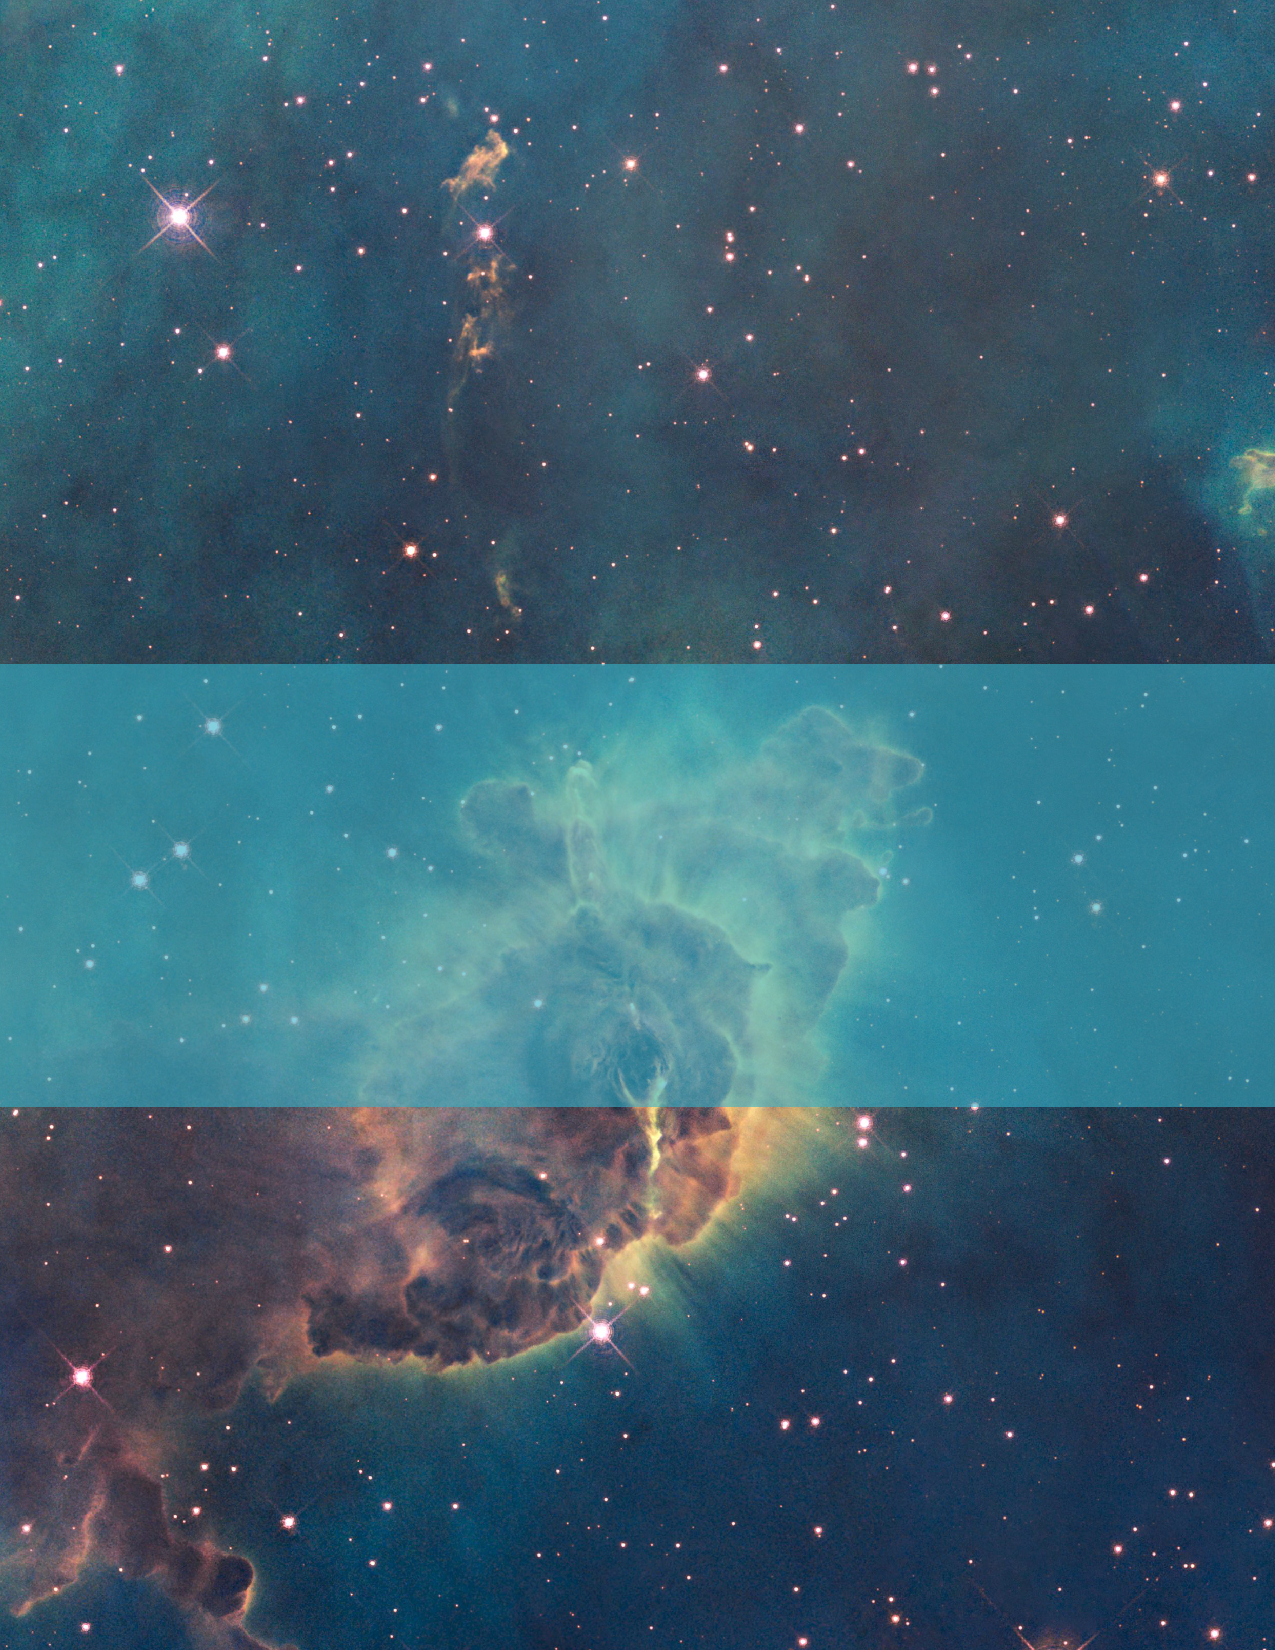
\includegraphics[scale=1.25]{esahubble}}} % Image background
	\centering
	\vspace*{5cm}
	\par\normalfont\fontsize{35}{35}\sffamily\selectfont
	\textbf{Simple Harmonic Oscillator (SHO)}\\
	{\LARGE Making The Way to Physics Easier}\par % Book title
	\vspace*{1cm}
	{\Huge Asif Ikbal}\par % Author name
	\endgroup
	
	%----------------------------------------------------------------------------------------
	%	COPYRIGHT PAGE
	%----------------------------------------------------------------------------------------
	
	\newpage
	~\vfill
	\thispagestyle{empty}
	
	%\noindent Copyright \copyright\ 2014 Andrea Hidalgo\\ % Copyright notice
	
	%\noindent \textsc{Summer Research Internship, University of Western Ontario}\\
	
	%\noindent \textsc{github.com/LaurethTeX/Clustering}\\ % URL
	
	%\noindent This research was done under the supervision of Dr. Pauline Barmby with the financial support of the MITACS Globalink Research Internship Award within a total of 12 weeks, from June 16th to September 5th of 2014.\\ % License information
	
	%\noindent \textit{First release, August 2014} % Printing/edition date
	
	%----------------------------------------------------------------------------------------
	%	TABLE OF CONTENTS
	%----------------------------------------------------------------------------------------
	
	\chapterimage{head1.png} % Table of contents heading image
	
	\pagestyle{empty} % No headers
	
	\tableofcontents % Print the table of contents itself
	
	%\cleardoublepage % Forces the first chapter to start on an odd page so it's on the right
	
	\pagestyle{fancy} % Print headers again
	
	
	\chapterimage{head2.png} % Chapter heading image
%\usepackage{physics}

\newpage
\section{Simple Harmonic Oscillator (SHO)}
\subsection{What is SHO?}
	Start with a spring resting on a horizontal, frictionless (for now) surface. Fix one end to an unmovable object and the other to a movable object. Start the system off in an equilibrium state — nothing moving and the spring at its relaxed length.

	Now, disturb the equilibrium. Pull or push the mass parallel to the axis of the spring and stand back. You know what happens next. The system will oscillate side to side (or back and forth) under the restoring force of the spring. (A restoring force acts in the direction opposite the displacement from the equilibrium position.) If the spring obeys Hooke's law (force is proportional to extension) then the device is called a simple harmonic oscillator (often abbreviated sho) and the way it moves is called simple harmonic motion (often abbreviated shm).

	A simple harmonic oscillator is an oscillator that is neither driven nor damped. It consists of a mass m, which experiences a single force F, which pulls the mass in the direction of the point x = 0 and depends only on the mass's position x and a constant k. Balance of forces (Newton's second law) for the system.
	

	\begin{equation}
	F=ma=m\frac{d^2x}{dt^2} = m\ddot{x} = -kx
	\end{equation}
	Solving this differential equation, we find that the motion is described by the function
	\begin{equation}
	x(t)= A \cos(\omega t + \varphi)
	\end{equation}
	\begin{equation}
	where \ \ \omega = \sqrt{\frac{k}{m}}
	\end{equation}
	
	As long as the system has no energy loss, the mass continues to oscillate. Thus simple harmonic motion is a type of periodic motion. Note if the real space and phase space diagram are not co-linear, the phase space motion becomes elliptical. The area enclosed depends on the amplitude and the maximum momentum.
	
	
	
		
\subsubsection{Example}






\section{mass spring system}

	mass = m \\
	distance form equilibrium x \\
	spring constant k \\
	Hook's law [F = -kx] \\
	force is proportional to the displacement \\
	\\
	unit 
	[F] = newton = $MLt^{-2}$ \ \ \ \ | m = mass 
	
	[x] = meter  = L \ \ \ \ \ \ \ \ \ \ | L = length 
	
	[x] = $\frac{MLt^{-2}}{L} = ML^{-2} $ | t = time
	
	newton law, [ F = ma = m$\ddot{x}$]\\
	since no offer force is action on the spring
	
	[$m\ddot{x}$ = -kx] this is the equation of motion(EOM) of a mass spring system.\\
	
	



\subsection{equation of motion (EOM)}
	


\subsection{solution of EOM}

	\begin{align}
		m\ddot{x} = -kx \\
		=> \ddot{x} = -\frac{k}{m}x \\
		=>\frac{d^2x}{dt^2} = -\omega^2 x\\
	\end{align}
	
	Assume the solution is, $x(t) = Ae^{-i\omega t}+Be^{-i\omega t} = x_1(t)+x_2(t)$ --->(trial) \\
	
	\textbf{Checking for $x_1(t)$}
	1.
	\begin{align}
		\frac{d^2x_1(t)}{dt^2} \\
		= A\frac{d^2}{dt^2}e^{i\omega t} \\
		= A\frac{d}{dt}\big(\frac{de^{i\omega t}}{dt}(i\omega)\big) \\
		= A (i \omega)\frac{d}{dt}e^{i\omega t} \\
		= A (i\omega) e^{i\omega t} (i\omega) \\
		= A (i\omega)^2 e^{i\omega t} \\
		= i^2\omega^2 Ae^{i\omega t} \\
		= - \omega^2 x_1(t)  \\
	\end{align}
	
	\textbf{Checking for $x_2(t)$}
	2.
	\begin{align}
		\frac{d^2 x_2(t)}{dt^2} \\
		= (-i\omega)^2 Be^{-i\omega t} \\
		= (-i\omega)^2 x_2(t) \\
		= (-\omega)^2 x_2(t) \\
	\end{align}
	constant A and B is determined form boundary condition.
	


\subsection{graph and calculation  of position}




\subsection{velocity}



\subsection{energy}



\section{simple pendulum}



\subsection{equation of motion (EOM)}



\subsection{solution of EOM}



\subsection{graph and calculation of position}



\subsection{velocity}



\subsection{energy}



\section{lagrangian for mass-spring and pendulum}

	\textbf{Lagrangian}	\\
	1.
	\begin{align}
		L = T - V \ \ (Definition)\\
		T = \ Kinetic \ energy \\
		V = \ potential \ energy \\
		and \ L = L(q,\dot{q}, t) \\
		q = \ generalized \ coordinate \\
		\dot{q} = \ generalized \ velocity \\
		t = \ time \\ 
		equation \ of \ motion \ or \ euler \ - \ lagrage \ EOM \\
		\frac{d}{dt}\bigg(\frac{\partial L}{\partial \dot{q}}\bigg) - \frac{\partial L}{\partial q} = 0 \\
	\end{align}
	
	\textbf{Lagrangian apporch for mass spring system} \\
	1.
	\begin{align}
		T = \frac{1}{2}mx^2 \\
		V = \frac{1}{2}kx^2 \\
		L = T - V \\
		= \frac{1}{2}m\dot{x}^2 - \frac{1}{2}kx^2 \\
		here: \\
		q= x \\
		q = \dot{x} \\
		\frac{\partial L}{\partial \dot{x}} = m\dot{x} \\
		EOM:\\
		\frac{d}{dt}\bigg(\frac{\partial L}{\partial \dot{x}}\bigg) = 0 \\
		=>\frac{d}{dt}(mx)+kx = 0 \\
		=>m\ddot{x}+kx \\
		=>\ddot{x}+\frac{k}{m}x = 0 \\
		=>\ddot{x}+\omega^2x = 0 \ ; \ \omega^2 = \frac{k}{m}
	\end{align}
	
	
	
	
	
	
	\textbf{Lagrangian}
	\begin{equation}
		Lagrangian = L = KE - PE = T - V
	\end{equation}
	KE and T is kinetic energy \\
	PE and V =  potential energy \\
	Equation Of motion can be determined by: \\
	Where X and X represented velocity and potion in generalized coordinate.\\
	let $v = x$ and $y = x$ \\
	\begin{equation}
	KE = \frac{1}{2}m\dot{x}^2 \ \ \ \ \ \ PE = mgx
	\end{equation}
	\begin{equation}
		L = KE - PE = \frac{1}{2}m\dot{x}^2 - mgx
	\end{equation}
	\begin{equation}
		\frac{\partial L}{\partial x} = 0 - mg
	\end{equation}
	\begin{equation}
	\frac{\partial L}{\partial \dot{x}} = m\dot{x} - 0
	\end{equation}
	\begin{equation}
		\frac{d}{dt}\bigg(\frac{\partial L}{\partial x}\bigg) = \frac{d}{dt}(m\dot{x}) = m \ddot{x}
	\end{equation}
	object on free fall...
	\begin{align}
		\frac{d}{dt}\bigg(\frac{\partial L}{\partial \dot{x}}\bigg) - \frac{\partial L}{\partial x} = 0 \\
		m\ddot{x} - (-mg) = 0 \\
		m\ddot{x}+mg = 0 \\
		\ddot{x} + g = 0 \\
		\ddot{x } = - g \\
		 a = - 9.8 m/s^2
	\end{align}
	
	
	
	
	
	
	\textbf{Simple pendulum} \\
	(1) Bob = small ball \\
	(2) thread or string of length l \\
	vertical line is the equilibrium: $h = l-l\cos\theta$
	potential energy, $v = mgh$ \\
	$v = mgh(1-\cos\theta)$ \\
	kinetic energy, $t = \frac{1}{2}m\dot{x}^2$ \\
	Lagrangian $L=T-V=\frac{1}{2}m\dot{x}^2-mgh(1-\cos\theta)$ \\
	variable --->x and $\theta$ \\
	$L=\frac{1}{2}m(l\theta)^2 - mgh(1-\cos\theta); \ variable \  is \ only \ \theta$ \\
	$\frac{d}{dt}\bigg(\frac{\partial L}{\partial\theta}\bigg) - \frac{\partial L}{\partial\theta} = 0\  EL \ equation $\\
	EL equation gives, \\
	\begin{align}
		\frac{d}{dt}(ml^2\dot{\theta})- (mgl\sin\theta) = 0 \\
		=>ml^2\ddot{\theta} + mgl\sin\theta = 0 \\
		=>\ddot{\theta} + \frac{g}{l}\sin\theta = 0 \\
		=>\ddot{\theta} + \frac{g}{l}\theta = 0 ;\ for \ small \ \theta \\
		=> \ddot{\theta} + \omega^2\theta = 0 ; \ \omega^2=\frac{g}{l} \\
	\end{align}
	Exactly like spring system \\ \\
	solution. \\
	\begin{align}
		\theta(t) = Ae^{-i\omega t} \\
		= A[\cos(\omega t)- i \sin(\omega t)] \\
		Taking \ only \ real \ port. \\
		\theta t = A\cos(\omega t) \\
		angular \ frequency ,\ \omega = \sqrt{\frac{g}{l}} \\
		\omega = \frac{2\pi}{T} = 2\pi t \\
		\frac{2\pi}{T}\sqrt{\frac{g}{l}} \\
		T = 2\pi\sqrt{\frac{l}{g}} \\
		=> T^2 = 4\pi^2\frac{l}{g} \\
		=> g = \frac{4\pi^2l}{T^2} \\
	\end{align}
	simply by meaning l and T we can find gravitational acceleration g!! and. \\
	$g= 9.8ms^{-2}$ \\
	$= 9.8m/s^2$ \\
	$= 32f/s^2$ \\
	
	\textbf{Newtonian approach(using force)} \\
	Lagrangian approach using energy better and general and suitable for complex system.\\
	\begin{align}
		F = ma \\
		ma = -Fg \sin\theta \\
		=>ma = -mg\sin\theta \\
		=>\ddot{\theta} = - \frac{g}{l}\theta \\
		=>\ddot{\theta}+\frac{\theta}{l}\theta = 0 \\
		=>\ddot{\theta}+\omega^2\theta=0 \\
		Solution\ \theta(t) = Ae^{-i\omega t} \\
		=> A \cos(\omega t) \\
	\end{align}
	
	
	



\subsection{EOM from lagrangian}









	%\input{Chapter2/chapter2.tex}

	
	
	
	
	
	
\end{document}